\section{Methods}\label{sec:methods}

Figure~\ref{fig:pipeline} summarises the pipeline. Every method maps a product text to one
of the \NLabelsInScope{} in-scope items or \textsc{oos}, with a calibrated confidence; some
may abstain.

\begin{figure}[t]
\centering
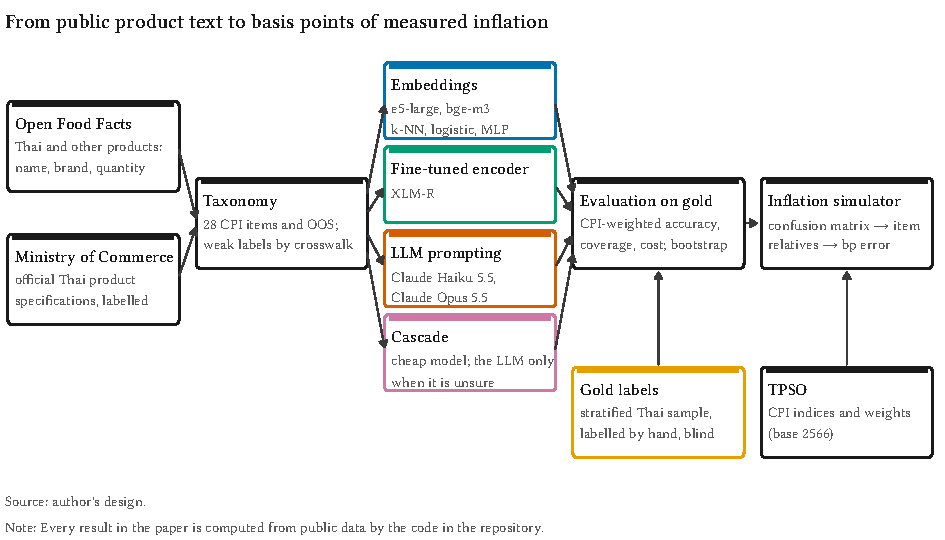
\includegraphics[width=\textwidth]{fig01_pipeline.pdf}
\caption{\textbf{The pipeline runs from public product text to basis points of measured
inflation.} Data sources (left) feed a taxonomy and weak labels, four families of classifier,
an evaluation on hand-labelled gold data and the inflation simulator. Source: author's
design.}
\label{fig:pipeline}
\end{figure}

\subsection{Classifiers}

\paragraph{Frozen multilingual embeddings.} Following Spectrum's design \citep[pp.~3, 19--20]{bis2026spectrum}, the
first family embeds each text once and trains a light classifier on the vectors.
We use two open multilingual embedding models run locally, \NameEfive{}
\citep[\texttt{\HfEfive};][]{wang2024me5} and \NameBge{} \citep[\texttt{\HfBge};][]{chen2024bgem3}.
On top of each we fit three classifiers: cosine $k$-nearest neighbours with
similarity-weighted votes, $k \in \{\CfgKs\}$ chosen on validation macro recall; multinomial
logistic regression; and a one-hidden-layer perceptron (\CfgMLPHidden{} units, dropout
\CfgDropout). The last two share one trainer: Adam with learning rate \CfgLR{} and weight
decay \CfgWeightDecay, class weights proportional to the inverse square root of class
frequency, and early stopping on validation loss (patience \CfgPatience).

\paragraph{Fine-tuned encoder.} XLM-R base \citep[\texttt{\HfXlmr};][]{conneau2020xlmr} with a
classification head, fine-tuned end to end on the same training pools with the same class
weights and early stopping (\CfgFtEpochs{} epochs at most, batch \CfgFtBatch, AdamW at
\CfgFtLR{} with linear warm-up and decay, inputs truncated to \CfgFtMaxLen{} tokens).

\paragraph{LLM prompting.} Two models of different cost, \NameOpus{} and \NameHaiku{}, through
the Anthropic API, one product per request. A fixed system prompt gives the instructions, the
item list grouped by CPI group with short descriptions grounded in TPSO's item headings, and
\CfgFewShot{} official specifications per item drawn from the training split
(Appendix~\ref{app:prompt}). The answer is constrained by a JSON schema: the model names the
group, then an item inside it, and a verbalised confidence, the probability in per cent that the item is right. Refusals count as
abstentions. Every response is cached and every billed call is logged with its tokens and
cost; total spend was capped at USD~\CfgCapUSD{} and came to USD~\LLMSpendUSD.

\paragraph{Cascade.} A cheap classifier answers when its calibrated confidence is at least a
threshold $t$; otherwise the product is routed to an LLM. We pair the cheap classifiers with
each LLM. For each pair, $t$ is the threshold with the highest weighted accuracy on the Thai
weak-label validation split, with ties broken by lower cost. It is fixed before the
reference set is touched, which then scores that one threshold.

\paragraph{Training data and the learning curve (RQ1).} Each embedding classifier is trained
on a sequence of pools: non-Thai weak labels only (zero-shot cross-lingual transfer to Thai);
plus Thai weak labels; plus $n \in \{\CfgBudgets\}$ or all official Thai labels; and official
labels alone. The budget $n$ counts every official label a run touches, validation included,
so a small-budget run cannot tune on thousands of extra official labels.

\paragraph{Calibration.} Each run's logits are divided by one scalar temperature fitted on its
own validation rows by negative log-likelihood \citep{guo2017calibration}; for $k$-NN the
logits are log vote shares. The calibrated top-class probability is the confidence used by
the coverage frontier and the cascade.

\subsection{Evaluation}

\paragraph{Expenditure-weighted accuracy.} What matters for a price index is not how many
products are classified correctly but how much CPI weight is measured correctly. Let $w_k$ be
the CPI weight of item $k$ and $r_k$ the recall of item $k$ on the reference set, estimated
with the design weights $1/\pi_i$ of Section~\ref{sec:ref} \citep{horvitz1952}. The headline
metric is
\begin{equation}
\mathrm{acc}_w = \frac{\sum_k w_k\, r_k}{\sum_k w_k}, \qquad
r_k = \frac{\sum_{i:\, y_i = k} \mathbb{1}[\hat y_i = k]/\pi_i}{\sum_{i:\, y_i = k} 1/\pi_i},
\label{eq:accw}
\end{equation}
the CPI-weighted mean recall over the evaluated items, a weighted version of Spectrum's
in-class recall \citep[p.~22]{bis2026spectrum}. We also report accuracy over the whole
held-out list, which counts \textsc{oos} specifications, and macro-F1. Abstentions are
errors at full coverage.

\paragraph{Coverage, cost and uncertainty.} Sweeping a confidence threshold traces a
weighted accuracy--coverage frontier \citep{geifman2017selective}: the CPI-weighted share of
products answered against $\mathrm{acc}_w$ on those. Cost per million products is the measured
mean API cost per call plus local compute at an assumed USD~\CfgGpuUSDHour{} per GPU-hour times
measured seconds per item. All intervals come from \CfgBoot{} bootstrap resamples of the
reference set, stratified by item \citep{efron1993bootstrap}. Method comparisons are
paired: every method is scored on the same resamples, and the comparisons were fixed in
code before the reference set was scored.

\subsection{From confusion matrices to basis points (RQ3)}\label{sec:sim}

\paragraph{Setting.} For an aggregate $A$ with member items $i$, the Lowe index satisfies
\begin{equation}
\frac{I_{A,t}}{I_{A,L}} = \sum_{i \in A} \frac{w_i}{W_A}\, R_{i,t}, \qquad
R_{i,t} = \frac{I_{i,t}}{I_{i,L}},
\label{eq:lowe}
\end{equation}
where $L$ is the price reference month, $w_i$ are price-updated weights and
$W_A = \sum_{i\in A} w_i$. We take the official item relatives $R_{i,t}$ as the true price
movement of every product in item $i$. This isolates the error due to classification: a
real web-price index would add sampling, matching and quality-adjustment error on top.

\paragraph{Misclassification.} Let $n_k$ be the universe share of products whose true item is
$k$ and $P$ a method's confusion matrix, $P_{kj}$ the probability that a product of item $k$
is classified as $j$. Item $j$ is then measured from a mixture of the products sent to it:
\begin{equation}
\tilde R_{j,t} = \sum_k \phi_{kj}\, R_{k,t}, \qquad
\phi_{kj} = \frac{n_k P_{kj}}{\sum_{k'} n_{k'} P_{k'j}}.
\label{eq:mix}
\end{equation}
Products sent to \textsc{oos} or abstained on are dropped. If nothing flows into an item, its
weight is redistributed within its CPI group; true \textsc{oos} products that leak into an
item move with the official non-food index. Out-of-scope items are measured perfectly. The
measured index is
\begin{equation}
\hat I_{A,t} = I_{A,t} + I_{A,L} \sum_{j \in A} \frac{w_j}{W_A}
\bigl(\tilde R_{j,t} - R_{j,t}\bigr),
\label{eq:measured}
\end{equation}
and the error is reported in basis points of month-on-month and year-on-year inflation for
the headline, food and core indices. A perfect classifier gives $\tilde R = R$ and reproduces
every official series exactly, which is a unit test of the code.

\paragraph{Product universe.} The shares $n_k$ are not observed: the reference set is the
office's list, not a stream of products. We state them as an assumption and report two
universes. In the primary one, products arrive in proportion to CPI expenditure weights,
with the weight outside the evaluated items arriving as out-of-scope products; in the
alternative they arrive in proportion to the office's specification list, that is, the
design-weighted shares of the reference set. In-scope items without specifications are held
at their official values, like out-of-scope items.

\paragraph{Decomposition.} Since $\sum_k \phi_{kj} = 1$,
$\tilde R_{j,t} - R_{j,t} = \sum_k \phi_{kj}(R_{k,t} - R_{j,t})$. The contribution of each
confusion $k \to j$ is therefore the item weight times the misallocated mass times the gap
between the two items' price movements. A confusion matters only if it is frequent, falls on
a heavily weighted item and joins items whose prices move differently.

\paragraph{Uncertainty.} The confusion counts come from the reference set. We draw
\CfgDraws{} confusion matrices from a
Dirichlet posterior, row by row. Sparse rows need a prior, and a flat one is not neutral: it
sends mass to arbitrary items and creates error even for a perfect classifier. We therefore
use an empirical-Bayes prior worth $\alpha = \CfgAlpha$ product per row, whose mean puts the
method's pooled accuracy on the diagonal and spreads the rest over the columns where that
method's errors actually go. Under this prior a perfect classifier has zero error in every
draw. Two variants bracket the result: a perfect classifier on the same universe (any error
left is due to coverage alone) and the method's matrix plus product-level sampling noise,
in which each product's log price drifts from its item's as a random walk with an assumed
annual standard deviation of \CfgSigmaLo\% or \CfgSigmaHi\%, and item $j$ averages the products
sent to it, the size of the held-out list standing in for the number of products.
